\documentclass[tikz]{standalone}
\usepackage{tikz}
\usetikzlibrary{patterns,snakes}
 
\begin{document}
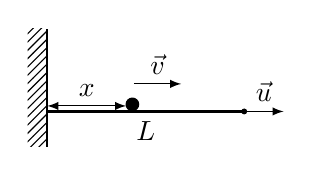
\begin{tikzpicture}

	\draw [draw=none, pattern=north east lines] (0,0.3) rectangle (-0.25,1.8);
	\draw [thick] (0,0.3) -- (0,1.8);
	\draw [arrows={-latex}] (1.1, 1.1) -- (1.7, 1.1) node [midway, above]  {$\vec{v}$};
	\draw [thick] (0, 0.75) -- (2.5,0.75) node [midway, below] {$L$};
	\draw [arrows={-latex}] (2.5, 0.75) -- (3.0, 0.75) node [midway, above]  {$\vec{u}$};
	\draw [fill] (2.5, 0.75) circle (0.03);
	\draw [arrows={latex-latex}] (0, 0.82) -- (1.0, 0.82) node [midway, above]  {$x$};
	\draw [fill] (1.08, 0.84) circle (0.08);

\end{tikzpicture}
\end{document}